\chapter{Authenticating Aggregate Queries over Set-Valued Data}\label{chap:aggregate-queries}

In this chapter, we investigate the problem of authenticating aggregate queries over set-valued data.

\section{Problem Formulation}\label{sec:aggregate-queries:problem}

A DO owns a dataset $\mathbb{D} = \{o_1, o_2, \dots, o_n\}$. Each object $o_i$ is represented by $\langle A_i, X_i \rangle$, where $A_i$ is a set of non-sensitive attributes, and $X_i$ is a sensitive multiset of \emph{features} (hereafter called \emph{feature set}). The DO outsources $\mathbb{D}$ to SP, together with an ADS signed with the DO's private key. Based on this, the SP provides aggregate query services to clients (e.g., \textbf{Q1} and \textbf{Q2}, and \textbf{Q3} in \Cref{example:intro:pgp}).

\textbf{Multiset Operations.} A multiset is a generalization of a set in which elements are allowed to occur more than once~\cite{TAOCP}. The number of occurrences is called the \emph{multiplicity} of an element. For instance, in multiset $\{a, a, b\}$, $a$ has a multiplicity of $2$ and $b$ has a multiplicity of $1$. The multiset is order insensitive, so it can be represented as a set of pairs $(x, \eta)$ where $x$ is an element and $\eta$ is its multiplicity. The above multiset $\{a,a,b\}$ can thus be rewritten as $\{(a,2), (b,1)\}$.
The most important operations in a multiset are \emph{union} and \emph{sum}, denoted as $\cup$ and $\uplus$, respectively. The \emph{union} operation on multisets is exactly the same as that on regular sets --- it simply unifies two multisets and sets the multiplicity of each element to 1. For instance, given multisets $X_1 = \{(a, 2), (b,1)\}, X_2 = \{(b,1), (c, 2)\} $, we have $X_1 \cup X_2 = \{(a,1)$, $(b,1)$, $(c,1)\}$. In contrast, the \emph{sum} operation sets the multiplicity of each element as the sum of multiplicities in the original multisets. For instance, given the same multisets as above, we have $X_1 \uplus X_2 = \{(a, 2)$, $(b, 2)$, $(c, 2)\}$.

\begin{figure}[t]
  \centering
  \begin{subfigure}[b]{.5\linewidth}
    \centering
    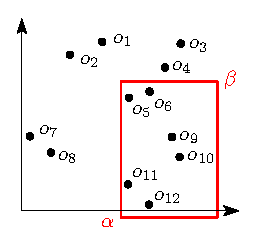
\includegraphics[width=.7\linewidth]{figs/aggregate-queries/example-object.eps}
    \caption{Objects}\label{fig:aggregate-queries:example:object}
  \end{subfigure}~%
  \begin{subfigure}[b]{.5\linewidth}
    \centering
    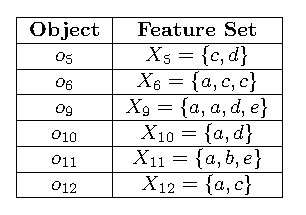
\includegraphics[width=.9\linewidth]{figs/aggregate-queries/example-feature.eps}
    \caption{Features}\label{fig:aggregate-queries:example:feature}
  \end{subfigure}
  \caption{Example of Aggregate Queries}\label{fig:aggregate-queries:example}
\end{figure}

\textbf{Aggregate Queries.} Since the results of aggregate queries are derived from aggregates of data, our study mainly focuses on the following primitive aggregate queries: \emph{max/min}, \emph{count}, \emph{sum}, \emph{top-$k$}, and \emph{frequent feature query (FFQ)}.\footnote{Extension to other more advanced aggregate queries such as \emph{average} and \emph{confidence} will be discussed in \Cref{sec:aggregate-queries:extension}.}  More specifically,  an aggregate query can be expressed in the form of $Q = (q, \{x_i\}, [\alpha, \beta])$, where $q$ is the aggregate operator, $\{x_i\}$ is the queried feature (which is only needed for \emph{count} and \emph{sum}), and $[\alpha, \beta]$ specifies the selection range on the non-sensitive attributes. Consider a sample query $Q = (q, \{x_i\}, [\alpha, \beta])$ in \Cref{fig:aggregate-queries:example}. The query range $[\alpha, \beta]$ selects the objects $o_5, o_6, o_9, o_{10}, o_{11}, o_{12}$. Since $X _5 \uplus X_6 \uplus X_9 \uplus X_{10} \uplus X_{11} \uplus X_{12} = \{(a, 6), (b, 1), (c, 4), (d, 3), (e, 2)\}$, the query result is based on the aggregate operator $q$, as follows:
\begin{itemize}
  \item $q=sum$ or $count$: This sums or counts the multiplicities of $\{x_i\}$ in all selected objects. Supposing $\{x_i\} = \{a\}$, the $sum$ and $count$ results are $(a, 6)$ and $(a, 4)$, respectively.\footnote{The $sum$ and $count$ results will be the same if there are no duplicate elements in the feature sets.}
  \item $q=max$ or $min$: This selects the feature with the maximum or minimum summed multiplicity in all selected objects. If $q=max$, the result is $(a, 6)$; if $q=min$, the result is $(b, 1)$. % chktex 35
  \item $q=$ \emph{top-$k$}: This selects the top-$k$ features with the largest summed multiplicities in all selected objects. Supposing $k$ = 3, the result is $(a, 6), (c, 4), (d, 3)$.
  \item $q=$ \emph{FFQ$_\delta$}: This selects the features whose summed multiplicities in all selected objects are no less than a threshold $\delta$. Supposing $\delta$ = 4, the result is $(a, 6), (c, 4)$.
\end{itemize}

The aggregate queries in \Cref{example:intro:pgp} can be reduced to the above aggregate queries as follows. \textbf{Q1} is simply a $max$ query, i.e., $(max, -, [95014, 95014])$. \textbf{Q2} is a \emph{count} query, i.e., $(count, \{\text{R-G1886S}\}, [00000, 99999])$. \textbf{Q3} is an FFQ query, $(FFQ_3, -, [20000, 29999])$, which finds the set of genes whose sum result is no less than 3. % chktex 35

\textbf{Threat Model and Problem Statement.} We consider two potential security threats:
\begin{inlineenum}
\item the SP could provide unfaithful query execution, thereby returning incorrect or incomplete query results; and
\item data privacy could be breached if sensitive source data are disclosed to the query client.
\end{inlineenum}
Thus, the authentication problem we are investigating is for the query client to verify that the SP executes $Q$ faithfully in terms of the following conditions:
\begin{inlineenum}
\item the candidate objects are correctly selected and no objects in the selection range are skipped;
\item the returned features and multiplicities are not tampered with; and
\item the query result satisfies the aggregation semantics.
\end{inlineenum}
The confidentiality requirement in this problem is to protect the objects' (sensitive) feature sets against the query client. That is, the client cannot infer the features (as well as their multiplicities) of any single object beyond what is implied from the query result.

If neither efficiency nor confidentiality is a concern, authenticating an aggregate query can work as follows. The SP returns a VO to the client, along with the query result. As a naive solution, the VO may include the non-sensitive attributes and sensitive features of all objects in $\mathbb{D}$ and a signature of $\mathbb{D}$. The client uses the VO to verify the soundness and completeness of the results by testing the following conditions:
\begin{itemize}
  \item None of the objects in $\mathbb{D}$ is tampered with.
  \item All candidate objects are in $[\alpha, \beta]$ and no objects in $[\alpha, \beta]$ are missing.
  \item The features and multiplicities of the candidate objects are correct.
  \item The result  satisfies the aggregation semantics of $q$.
\end{itemize}

However, the verification cost of this naive solution is prohibitively high because the entire dataset has to be returned. Moreover, verifying the last two conditions without disclosing sensitive feature sets requires privacy-preserving protocols. To address these issues, we propose an efficient privacy-preserving authentication framework based on verifiable multiset operations, the preliminaries of which are introduced in the next section.

\section{Preliminaries}\label{sec:aggregate-queries:prelim}

This section gives some preliminaries on cryptographic constructs and integrity assurance.

\textbf{Cryptographic Hash Function.}
A cryptographic hash function $H(\cdot)$ accepts an arbitrary-length string as its input and returns a fixed-length bit string. It is collision resistant, i.e., it is difficult to find two different messages $m_1$ and $m_2$ such that $H(m_1) = H(m_2)$. Classic cryptographic hash functions include SHA-1, SHA-2, and SHA-3.

\textbf{Bilinear-Map (BM) Accumulator.} This maps a multiset to a single value for ease of processing. Let $\mathbb{G}$ be a cyclic multiplicative group of order $p$. A BM accumulator is a function of a multiset $X$ of $n$ elements in the cyclic group $\mathbb{Z}_p$~\cite{10.1007/978-3-540-30574-3_19}. It returns an \emph{accumulative value} of $X$:
\begin{align}
  acc(X) = g^{P(X)} = g^{\prod_{x\in{X}}{(x+s)}},
\end{align}
where $g$ is a group generator of $\mathbb{G}$, $s \in \mathbb{Z}_p^* = \mathbb{Z}_p\backslash\{0\}$ is a random secret, and $P(X) = \prod_{x\in{X}}{(x+s)}$.

One useful property of $acc(X)$ is that even without knowing $s$, $acc(X)$ can still be computed by $X$ and $g, g^s, \dots, g^{s^k}$ ($k \ge |X|$) through polynomial interpolation. As for its security, it has been proved in~\cite{10.1007/s00453-014-9968-3} that the accumulative function $acc(\cdot)$ is collision resistant.

\textbf{Randomized BM Accumulator.} The above accumulative value $acc(X)$ is deterministic for a fixed multiset $X$. As such, an adversary can determine with high confidence that two multisets are the same if they happen to have the same accumulative value. To enhance confidentiality, we propose  randomizing the $acc$ value of $X$ as
\begin{align}
  acc(X) = g^{P(X) \cdot r_X},\label{eqn:aggregate-queries:random-bm}
\end{align}
where $r_X$ is a random value hidden from the query client but disclosed to the SP\@. It is worth noting that this randomization does not affect the original properties of a BM accumulator. We will further prove in \Cref{sec:aggregate-queries:security-analysis} that the randomized $acc$ values are indistinguishable under chosen plaintext attack.

\textbf{Bilinear Pairing.} This maps a pair of elements in two groups to a single element in a third group. Let $\mathbb{G}_{t}$ be another cyclic multiplicative group with the same order $p$. We can find a bilinear mapping $e: \mathbb{G} \times \mathbb{G} \rightarrow \mathbb{G}_t$ which has the following properties:
\begin{enumerate}
  \item \emph{Bilinearity}: If $u, v \in \mathbb{G}$ and $e(u,v)\in\mathbb{G}_t$, then $e(u^{a}, v^{b}) = e{(u, v)}^{ab}$ for any $u,v$.
  \item \emph{Non-degeneracy}: $e(g, g) \neq 1$.
  \item \emph{Computability}: Given $u,v\in \mathbb{G}$, it is easy to compute $e(u, v)$.
\end{enumerate}

\textbf{Bilinear $q$-Strong Diffie-Hellman (DH) Assumption.} This assumption shows that bilinear pairing is appropriate for multiset operation authentication as it is hard to forge. Let $(\mathbb{G}, \mathbb{G}_t, e, g)$ be a bilinear pairing. This assumption says that as long as $s\in \mathbb{Z}_p^*$ is secret, even given all elements $g, g^s, \dots, g^{s^k} \in \mathbb{G}$, no probabilistic polynomial-time (PPT) algorithm can derive ${e(g,g)}^{1/(x+s)}$ for any $x\in \mathbb{Z}_p^*$ with a probability higher than a negligible value~\cite{10.1007/978-3-540-28628-8_3}. In essence, this bilinear $q$-strong DH assumption extends the regular DH assumption on $g$ and $\mathbb{G}$ to $e(g,g)$ and $\mathbb{G}_t$. This assumption will be used as a foundation in our security analysis.

\textbf{Set Operation Authentication.} Based on the above, two result verification protocols have been introduced in~\cite{10.1007/978-3-642-54631-0_7,10.1007/978-3-642-22792-9_6} to authenticate the following operations on two sets $X_1$ and $X_2$:
\begin{inlineenum}
\item $X_1 \subseteq X_2$ and~\label{enum:aggregate-queries:prelim:set1}
\item $X_1 \cap X_2 = \emptyset$.~\label{enum:aggregate-queries:prelim:set2}
\end{inlineenum}

For~\ref{enum:aggregate-queries:prelim:set1}, the server computes a witness value $W = acc(X_2 - X_1)$ and returns it to the query client. The client then verifies $X_1 \subseteq X_2$ by checking:
\begin{align*}
  e(acc(X_1), W) \stackrel{?}{=} e(acc(X_2), g).
\end{align*}

For~\ref{enum:aggregate-queries:prelim:set2}, according to the extended Euclidean algorithm, there are two polynomials $Q_1, Q_2$ such that
\begin{align*}
  Q_1 \cdot P(X_1) + Q_2 \cdot P(X_2) = 1.
\end{align*}
As such, the server prepares $F_1 = g^{Q_1}, F_2 = g^{Q_2}$, and then the client verifies it by checking:
\begin{align*}
  e(F_1, acc(X_1)) \cdot e(F_2, acc(X_2)) \stackrel{?}{=} e(g,g).
\end{align*}
Though these two protocols are privacy-preserving in nature and can be extended to multisets, we have yet to design privacy-preserving authentication protocols for other multiset operations such as \emph{sum} and \emph{union}, which will be covered in \Cref{sec:aggregate-queries:multiset-op}.

\section{PA$^2$: Privacy-Preserving Authentication Framework for Aggregate Queries}\label{sec:aggregate-queries:pa2}

\begin{figure}[t]
  \centering
  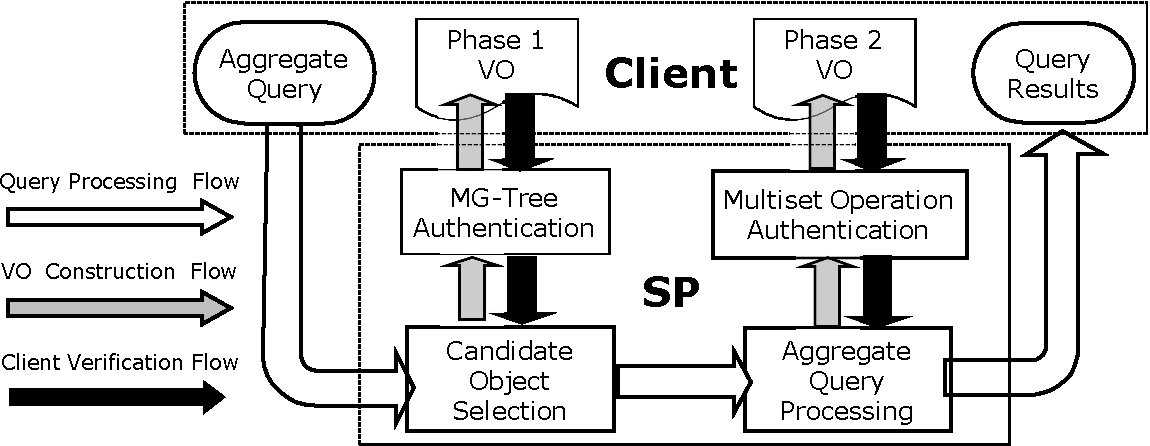
\includegraphics[width=.8\linewidth]{figs/aggregate-queries/overview.pdf}
  \caption{PA$^2$ Authentication Framework Overview}\label{fig:aggregate-queries:overview}
\end{figure}

In this section, we present the complete framework that can authenticate various aggregate queries while preserving data confidentiality. \Cref{fig:aggregate-queries:overview} illustrates both the query and authentication flow charts of the framework. The framework consists of two phases: candidate object selection and aggregate query processing. Recall that given an aggregate query $Q = (q, \{x_i\}, [\alpha, \beta])$, the SP first selects the candidate objects within the range $[\alpha, \beta]$, and then computes the aggregate values of these candidate objects with regard to the queried feature $x_i$. Along with query processing, the SP also constructs the VOs for both phases. Once the client receives the query results and VOs, it can authenticate the correctness of the entire query following the verification flow, which is the opposite of the SP's VO construction flow. In what follows, we present the detailed procedure of each phase in this framework, starting with the second phase for clarity reasons.

\subsection{Privacy-Preserving Authentication Protocols on Multiset Operations}\label{sec:aggregate-queries:multiset-op}

Before running into the detailed procedure of authenticating aggregate queries, we present five core privacy-preserving authentication protocols on multiset operations. The challenge is that the client cannot learn any sensitive feature information when authenticating the multiset operations. Inspired by~\cite{10.1145/2660267.2660373}, our key idea is to leverage the randomized bilinear-map accumulator $acc(\cdot)$ (i.e., \Cref{eqn:aggregate-queries:random-bm}) introduced in \Cref{sec:aggregate-queries:prelim} to hash a multiset into a fixed-length value with collision resistance. With the bilinear pairing function $e(\cdot,\cdot)$ (also introduced in \Cref{sec:aggregate-queries:prelim}), the client can verify the accumulated value of the output multiset without learning the content of each input multiset. This distinguishes the accumulator function from other cryptographic hash functions such as SHA-1.

In the rest of this section, we introduce the five core privacy-preserving authentication protocols on multiset operations, namely, $subset$, $sum$, $empty$, $union$, and $times$. For ease of presentation, we mark below any unverified value computed by the SP with $^*$, while all other unmarked values are trusted or already verified by the candidate object selection protocol (to be explained in \Cref{sec:aggregate-queries:grid}). We also assume that the seeds $g, g^s, \dots, g^{s^k}$ are public and that the random values $r_{X_i}$'s are known to the DO and SP but hidden from the client.

\textbf{Subset:} $sub(X_i, X_j)$.
Given two multisets $X_i, X_j$, it returns the accumulative value $acc(X_j-X_i)$. Note that if $X_i \nsubseteq X_j$, the SP cannot compute a correct value of $acc(X_j - X_i)$. Hence, if $acc(X_j-X_i)$ is verified as correct, the client is assured that $X_i \subseteq X_j$. The detailed protocol is as follows:
\begin{enumerate}
  \item The SP computes the accumulative value ${acc(X_j-X_i)}^*$ based on $X_i$, $X_j$, the random values $r_{X_i}$, $r_{X_j}$, and the public seeds $g, g^s, \dots, g^{s^k}$ (thanks to the nice property of $acc$ as mentioned in \Cref{sec:aggregate-queries:prelim}), and sends it to the client together with $acc(X_i)$ and $acc(X_j)$.
  \item The client verifies the correctness of ${acc(X_j-X_i)}^*$ by checking the following condition, where we exploit the property of bilinear pairing function  $e(\cdot,\cdot)$ as mentioned in \Cref{sec:aggregate-queries:prelim}.
    \begin{align*}
      e(acc(X_i), {acc(X_j-X_i)}^*) \stackrel{?}{=} e(acc(X_j), g).
    \end{align*}
\end{enumerate}

\textbf{Sum:} $sum(\{X_1, \dots, X_n\})$.
Given a set of multisets $\{X_1, \dots, X_n\}$, it returns the accumulative value $acc(S)$ of the sum set $S = \uplus \{X_i\}$. The detailed protocol is as follows:
\begin{enumerate}
  \item The SP computes the accumulative values ${acc(X_1 \uplus X_2)}^*$, ${acc(X_1 \uplus X_2 \uplus X_3)}^*$, $\dots$, ${acc(S)}^*$, and sends them to the client together with $acc(X_1)$, $\dots$, $acc(X_n)$.
  \item The client verifies the correctness of ${acc(S)}^*$ by checking the following equations one by one:
    \begin{align*}
      \left \{
        \begin{array}{l}
          e(acc(X_1), acc(X_2)) \stackrel{?}{=} e({acc(X_1 \uplus X_2)}^*, g)\\
          e({acc(X_1\uplus X_2)}^*, acc(X_3)) \stackrel{?}{=} e({acc(X_1\uplus X_2\uplus X_3)}^*, g) \\
          \vdots\\
          e({acc(\uplus_{i=1}^{n-1} X_i)}^*, acc(X_n)) \stackrel{?}{=} e({acc(S)}^*, g)
        \end{array}
      \right.
    \end{align*}
\end{enumerate}

\textbf{Empty:} $empty(\{X_1, \dots, X_n\})$.
Given a set of multisets $\{X_1, \dots, X_n\}$, it verifies whether $\cap \{X_i\} = \emptyset$. According to the extended Euclidean algorithm, if $\cap \{X_i\} = \emptyset$, there exist $n$ polynomials $Q_i$ such that $\sum_{i=1}^n Q_i \cdot P(X_i) = 1$. The detailed protocol is as follows:
\begin{enumerate}
  \item The SP computes $n$ values $F_i^* = g^{{Q_i}/{r_{X_i}}}$, and sends $F_1^*$, $\dots$, $F_n^*$, $acc(X_1)$, $\dots$, $acc(X_n)$ to the client.
  \item The client verifies the result is empty if the following equation holds:
    \begin{align*}
      \prod_{i=1}^n e(acc(X_i), F_i^*) \stackrel{?}{=} e(g, g).
    \end{align*}
\end{enumerate}

\textbf{Union:} $union(\{X_1, \dots, X_n\})$.
Given a set of multisets $\{X_1, \dots, X_n\}$, it returns the accumulative value $acc(U)$ of the union set $U = \cup_{i=1}^n X_i$. This operation is more complicated than the \emph{sum} operation. Denote $\widehat{X}_i$ as the set version of a multiset $X_i$. The client needs to verify two conditions:
\begin{enumerate}
  \item Deflation checking: $\widehat{X}_1 \subseteq U \wedge \widehat{X}_2 \subseteq U \wedge \cdots \widehat{X}_n \subseteq U$. This is to prevent the SP from deliberately missing any object;
  \item Inflation checking:$(U - \widehat{X}_1) \cap (U - \widehat{X}_2) \cap \cdots (U - \widehat{X}_n) = \emptyset$. This is to prevent the SP from deliberately adding any non-result object.
\end{enumerate}
We can authenticate them based on the above $sub$ and $empty$ protocols as follows:
\begin{enumerate}
  \item Use protocols $sub(\widehat{X}_1, U)$, $sub(\widehat{X}_2, U), \dots, sub(\widehat{X}_n, U)$ to verify the first condition. This not only authenticates $\widehat{X}_i \subseteq U$, but also provides the client the correct $acc(U-\widehat{X}_i)$.
  \item The SP computes a special hash value ${h_e(U)}^*$ of the union set $U$, and by verifying this value the client is assured that the SP knows the pre-image $U$ besides ${acc(U)}^*$.\label{enum:aggregate-queries:multiset-op:union:step2}
  \item Use protocol $empty(\{(U-\widehat{X}_1), (U-\widehat{X}_2), \dots, (U -\widehat{X}_n)\})$ to verify the second condition.
\end{enumerate}
In step~\ref{enum:aggregate-queries:multiset-op:union:step2}, $h_e(\cdot)$ is an \emph{extractable collision resistant hash} (ECRH) function that has one unique property --- extractability~\cite{10.1145/2090236.2090263}. By presenting a correct ${h_e(U)}^*$ value, the SP can prove that it knows $U$. Inspired by~\cite{10.1145/2090236.2090263}, we design $h_e(\cdot)$ for a multiset $X=\{x_1, x_2, \dots, x_t\}$ as follows:
\begin{align*}
  h_e(X) = (h_1, h_2) = (\prod_{i \in [t]} g^{s^i a_i}, \prod_{i \in [t]} g^{\alpha s^i a_i}),
\end{align*}
where $s, \alpha \in \mathbb{Z}_p^*$ are secret values only known to the DO of $X$, and $a_i$ is the $i^{th}$ coefficient for polynomial $P(X)\cdot r_X$. Before any other party can compute or verify $h_e(X)$, the DO releases $g, g^s, \dots, g^{s^k}, g^\alpha, g^{\alpha s}, \dots, g^{\alpha s^k} \in \mathbb{G}$ to the public, where $k \ge |X|$, the cardinality of $X$. Then any party, including the client, can verify whether a hash value $h_e(X)$ is correct by checking the following equations:
\begin{align*}
  e(h_e(X).h_1, g^\alpha) &\stackrel{?}{=} e(h_e(X).h_2, g), \\
  h_e(X).h_1 & \stackrel{?}{=} acc(X).
\end{align*}

\textbf{Times:} $times(X, t)$.
Given a multiset $X$ and a coefficient $t$, it returns the accumulative value $acc(t \cdot X)$ of $t \cdot X$, which raises the multiplicity of each element in $X$ by $t$. For example, if $X = \{(a, 2), (b, 3)\}$, then $3\cdot X = \{(a, 6), (b, 9)\}$. A straightforward solution is to use the $sum$ protocol directly as $sum(\{\overbrace{X, X, \dots, X}^{t}\})$. Here we give a more efficient solution using $sum$ on the binary components. Let $t = {(b_0b_1\cdots b_d)}_2$, the binary form of $t$. The client only needs to execute $sum(\{b_0 \cdot X, \dots, b_i \cdot 2^i \cdot X, \dots, b_d \cdot 2^d \cdot X\})$, where $b_i=1$. For instance, if $t = 5={(101)}_2$, then the client only executes $sum(\{X, 4\cdot X\})$. The detailed protocol is as follows:
\begin{enumerate}
  \item Let $d = \lfloor \log_2(t) \rfloor$, the SP computes ${acc(2\cdot X)}^*, \dots, {acc({2^d} \cdot X)}^*, {acc(t \cdot X)}^*$, and sends them to the client together with $acc(X)$.
  \item The client first verifies the values ${acc(2\cdot X)}^*, \dots, {acc({2^d} \cdot X)}^*$ by checking the following equations:
    \begin{align*}
      \left \{
        \begin{array}{l}
          e(acc(X), acc(X)) \stackrel{?}{=} e({acc(2\cdot X)}^*, g)\\
          e({acc(2\cdot X)}^*, {acc(2\cdot X)}^*) \stackrel{?}{=} e({acc(4 \cdot X)}^*, g) \\
          \vdots\\
          e({acc(2^{d-1} \cdot X)}^*, {acc(2^{d-1} \cdot X)}^*) \stackrel{?}{=} e({acc({2^d} \cdot X)}^*, g)
        \end{array}
      \right.
    \end{align*}
  \item The client then verifies ${acc(t \cdot X)}^*$ according to the binary form of $t(b_0b_1\cdots b_d)$.
\end{enumerate}

We will show in the cost analysis that this protocol significantly improves the performance over the straightforward $sum$ solution.
